%\documentclass[conference]{IEEEtran}
\documentclass[10pt,conference]{IEEEtran}
\IEEEoverridecommandlockouts
% The preceding line is only needed to identify funding in the first footnote. If that is unneeded, please comment it out.
\usepackage{cite}
\usepackage{amsmath,amssymb,amsfonts}
\usepackage{algorithmic}
\usepackage{graphicx}
\usepackage{textcomp}
\usepackage{xcolor}
\usepackage{url}
\usepackage{listings}
\usepackage{courier}
\usepackage{xspace}
\usepackage{multirow}
\usepackage{colortbl}
\usepackage{blindtext}
\usepackage{float}
\usepackage[font=scriptsize]{caption}
\usepackage[sort&compress,square,comma,authoryear]{natbib}
%\newcommand{\sd}[1]{\textbf{"\textsc{SD:}} \textit{#1}"}

\newcommand{\nnbb}[2]{
    \fbox{\bfseries\sffamily\scriptsize#1}
    {\sf\small$\blacktriangleright$\textit{#2}$\blacktriangleleft$}
   }
\newcommand{\sd}[1]{\nnbb{\textcolor{orange}{St\'{e}f}}{\textcolor{orange}{#1}\xspace}}
\newcommand{\hr}[1]{\nnbb{Henrique}{#1\xspace}}
\newcommand{\ap}[1]{\nnbb{\textcolor{blue}{Apierr}}{\textcolor{blue}{#1}\xspace}}
\newcommand{\Miner}[0]{Miner\xspace}
\newcommand{\Miners}[0]{Miners\xspace}
\newcommand{\miner}[0]{miner\xspace}
\newcommand{\miners}[0]{miners\xspace}
\newcommand{\gas}[0]{gas\xspace}
\newcommand{\Gas}[0]{Gas\xspace}
\newcommand{\Transaction}[0]{Transaction\xspace}

\newcommand{\SmartGas }[0]{\textsc{SmartGas}\xspace}

\newcommand{\eg}{\emph{e.g.,}\xspace}
\newcommand{\ie}{\emph{i.e.,}\xspace}
\newcommand{\etal}{\emph{et al.,}\xspace}
\newcommand{\ct}[1]{{\textsf{#1}}\xspace}
\usepackage[scaled=0.85]{helvet}

\def\BibTeX{{\rm B\kern-.05em{\sc i\kern-.025em b}\kern-.08em
    T\kern-.1667em\lower.7ex\hbox{E}\kern-.125emX}}
\begin{document}

\title{Improving practices in a medium french  company: First step}
% \title{Toward  maintainance of  a commencial software: Time serie model of defects }
%\thanks{Identify applicable funding agency here. If none, delete this.}}

\author{\IEEEauthorblockN{HOUEKPETODJI Mahugnon Honore\IEEEauthorrefmark{1}\IEEEauthorrefmark{2},
Nicolas Anquetil\IEEEauthorrefmark{3}}
\IEEEauthorblockA{\IEEEauthorrefmark{1}University of Lille, France}
\IEEEauthorblockA{\IEEEauthorrefmark{2}Inria Lille - Nord Europe, France}
homahugnon@gmail.com, nicolas.anquetil@inria.fr}


\maketitle

\begin{abstract}
Legacy systems are old software that still does useful tasks.
In industrial software companies, legacy systems are often crucial for the company business model and represent a long-term business investment.
Legacy systems are known to be hard to maintain.
This is the case in a french company whose main product is twenty years old software written in PowerBuilder.
Our long-term goal is to help it re-engineer this system.
But how to validate our intervention?
Little data is available on the system and specifically, past versions of the source code are not easy to recover.
This constrained us on the metrics we could use.
%We evaluate the maintenance state of the system and produce a dashboard to monitor our future actions.
In this paper, we present a lightweight model to characterize the situation of the system and allow us to monitor it in the future.
\end{abstract}

\begin{IEEEkeywords}
Legacy system, software quality model .
\end{IEEEkeywords}

\section{Introduction}
%-------------------------------------------------------------------------------

%Software companies usually invest time and energy to improve the quality of the software they develop to respond to the rising market demands.
Software companies have little spare resources to allocate to software quality improvement or code defect removal.
As a result they often develop features in a hurry.
As the system grows, it becomes harder and harder to maintain.
%Rewriting this software require time and a lot of resources.
To ensure the future of the system, and through it, of the company itself, some re-engineering actions might be necessary.
Long period of growth and evolution of the systems as well as staff evolution, lead to problems such as dead code, duplicate code, and obsolete documentation. 
The developers at the origin of the application are no longer present, so a large part of the knowledge (and this at different levels of granularity) is scattered or lost. 

This is the situation at CIM, a medium French company, which main business product we are studying.
The system is written in an old language (PowerBuilder) typically unknown to young programmers which translates in a difficulty to hire new developpers.
There is also a sense in the development team that the system suffers from architecture erosion and is difficult to maintain or evolve which translates into a steep learning curve for new developpers.
We are trying to help this company improve its software engineering practices and restructure the system to improve the situation.

In this paper, we are trying to answer the following question:
How to validate our intervention and can we measure its concrete impact on the system and its evolution?

%How to provides a report on the state of the system to the entire company?
For the reasons explained above, we cannot completely rely on current developers knowledge of the system.
The only usable information about the system is its non versioned source code and a ticket database.
Past literature often relied on historical data on the source code, for example
cyclomatic complexity \cite{gill91}, or number of lines of code \cite{port18}.
In lack of a reliable software versonning system, we could not use these solutions.

We mine and analyse the ticket database to overcome our problem.
This paper presents the results of this work.

 This paper is structured as follows: we start with related work in the section \ref{sec:related-work}, followed by  the section \ref{sec:defectModel}  in which we present ticket database mining background. 
 In the section 4 we present our results and validation. We  conclude in section 5.
 
\section{Related Work}
%-------------------------------------------------------------------------------
\label{sec:related-work}

"intro": de quoi on va parler et pourquoi en parler ?

%A software defect is a mistake at coding level, which manifests in a deviation from expected behavior. 
%Mining a software defect history helps to collect valuable information about the software life evolution. 
Software re-engineering monitoring should be supported by prediction models that predict the quality under control (\cite{Lenar17}). 

%Software defect history can be used alone to build a software defect model using statistical techniques or machine learning algorithms to predict post-release defects in software.

Software defect prediction has already been extensively discussed in literature in numerous publications.
This literature is summarised in many literature surveys: \cite{Catal09,Hall12,Hoss17,Li19a,malh15}.

Software defect history combined with static source code metrics and or developers metric to monitor maintenance quality.
For example \cite{gill91} used McCabe’s cyclomatic complexity metric divided by the size of the system to predict software maintenance productivity.
Dan Port and Bill Taber \cite{port18} use the number of  bugs difference between release, reported bugs per logical lines of code, number of day between releases, the system size change between release, the size change per day, the time spent  per bugs, test per logical line of code, comment per logical line of code to evaluate software development policy  to monitor maintenance quality of a software at Jet propulsion Laboratory.

"conclusion": (1) on ne veut pas faire de prediction (2) on n'a pas d'historique de code
donc: on develop notre propre analyse sur la ticket db.

\section{Defect Model}
%-------------------------------------------------------------------------------
\label{sec:defectModel}

\subsection{Moving average}
%-------------------------------------------------------------------------------

A moving average is a statistic technical usually used to smooth a time series data and estimate it trend \cite{MOLU17}.
 The moving average of a period m is a series of consecutive averages of m terms at a time. 
 The simple moving average is calculated as:

\begin{equation}
SMA_{t+1}=\frac{\sum\limits_{i=t-m}^t X_i}{m}
\end{equation}

\subsection{Presentation of the studied system}
%-------------------------------------------------------------------------------
Legacy systems have a lifespan of several decades, decisions made at the beginning of development and their evolution over the life of the software are often lost. 
This is the case of the studied system  which has more than 20 years. 
It's a 3 MLOC software written in Powerbuilder. With 117 Powerbuilder library, the  bigest library is  over 300 KLOC.
The system is not versioned and old versions are lost until 2012.

Powerbuilder is a programming language and integrated development environment initially developed by PowerSoft. The first version was published in 1992.
Powerbuilder applications components are grouped by libraries.  
A Powerbuilder library contains differents type of Objects: Datawindow, User object, Global function,  menu, etc. 
Powerbuilder is not totally object-oriented, as inheritance and object-oriented features are limited to some object types (Windows, Userobjects and Menus). 
Its version 2017 supports version control systems.% and the support is not stable. 
    

\subsection{Ticket}
%-------------------------------------------------------------------------------

A ticket is related do a task to do. 
This task can be fixing a defect, writing documentation, adding a new feature, etc. 
A ticket is open for a task . 
Once the task is done and validated, the ticket is close.
A ticket has the following characteristics:

\begin{itemize}
\item the libraries it  is related to
\item the creation date
\item the closing date
\item time spent by a developer
  \begin{itemize}
\item time to analyze
\item time to implement solution
\item time to test
  \end{itemize}
\item  the estimation of the time needed by the developer to work on the ticket
\end{itemize}
In this paper we use defect history  from tickets database to build a simple defect model that evaluate developers effort.

\section{Methodology}
%-------------------------------------------------------------------------------
\label{sec:methodology}

We collected data  from the company Tickets database .  
Then we proceed to data cleaning.
The data analytic process is guided by the following research methodology:
\begin{itemize}
\item Pose a problem
\item Make experimentation on data
\item Validation of results
\end{itemize}

\subsection{Data collection and data cleaning}
%-------------------------------------------------------------------------------

The ticket database contains data from 1998  until 2019. 
This data includes tickets  different teams and software in  the company. 
In the field related to the  library a ticket is related to,  the name of the library is not always well written. 

We use tickets database data from 2004 to 2019 . 
We  remove all tickets, not related  to the studied system and reformat duration per ticket.
By interviewing developers, we categorize tickets into two sets: tickets related to defects and tickets related to evolution.

 \subsection{Questions}
 \begin{itemize}
 \item How to avoid the system source code lost?
 \item What is the number of defect per library?
 \item How long on average, does it take to open and close a ticket?
 \item How long on average,  does a developer spend on a ticket ?
 \item How long on average, does a developer spend to test a ticket after development ?
 \item Does the team manager estimate well  the time needed by the developer?
 \item If the time estimated by the team manager is good, does the developer finish because  of time constraint?
 \end{itemize}
 
 \subsection{Experimentation}

\subsubsection{Avoid the system source code lost}
%-------------------------------------------------------------------------------

The system source code is not versioned.  Some versions of the system are lost. 
When developers work in the same version of the system, they chat with each other to notify which part of the system they are modifying so that others won't modify the same part to avoid losing modifications. Besides, each developer has to write in a comment in the source code his name and the date in the form of each modification he made.  We believe that writing author in a comment in the source can be easily handled by a version control system.
This is because of Powerbuilder support version controlling system from the 2017 release. 
The support provided by Powerbuilder is not stable.
The conflict resolution option is limited and a simple copy-paste of a library require a huge walk-around to update files. 
With this constraint, we chose to start with a simple to use version controlling system. We introduce Apache Subversion. 

 \subsubsection{Number of defects per library}
 %-------------------------------------------------------------------------------

We plot  defects and evolution per library over time.  In x axis we have years and in y axis  we have the number of defects  or evolution.
This give us an overview of defect  history per library. And  which libraries   trend to have defects.

\subsubsection{ Average time to open and close a ticket}
%-------------------------------------------------------------------------------

A ticket is closed when the task it is related to is done and validated. 
We use the time a ticket remains open over the life cycle of the studied system as an indicator of the system state. 
We grouped tickets by the month of creation.
We then compute the average of  the duration between the time when the ticket is created and the time when the ticket is closed for each month.  
We do this for tickets categorized as defect and tickets categorized as evolution. 
We finally plot the result of each category into a graph.  First, the plot exhibits rapid up-and-down variation.
We could not derive any trend from this variation. 
We smooth the plot using the simple moving average of period 4 on the data.  
We then plot the linear regression to fit the data.  
The figure \ref{fig:evol} presents the trend of time to close evolution ticket and  the figure \ref{fig:defect} shows  the trends  of time to close defects tickets.

\begin{figure}[H]
  \centering
  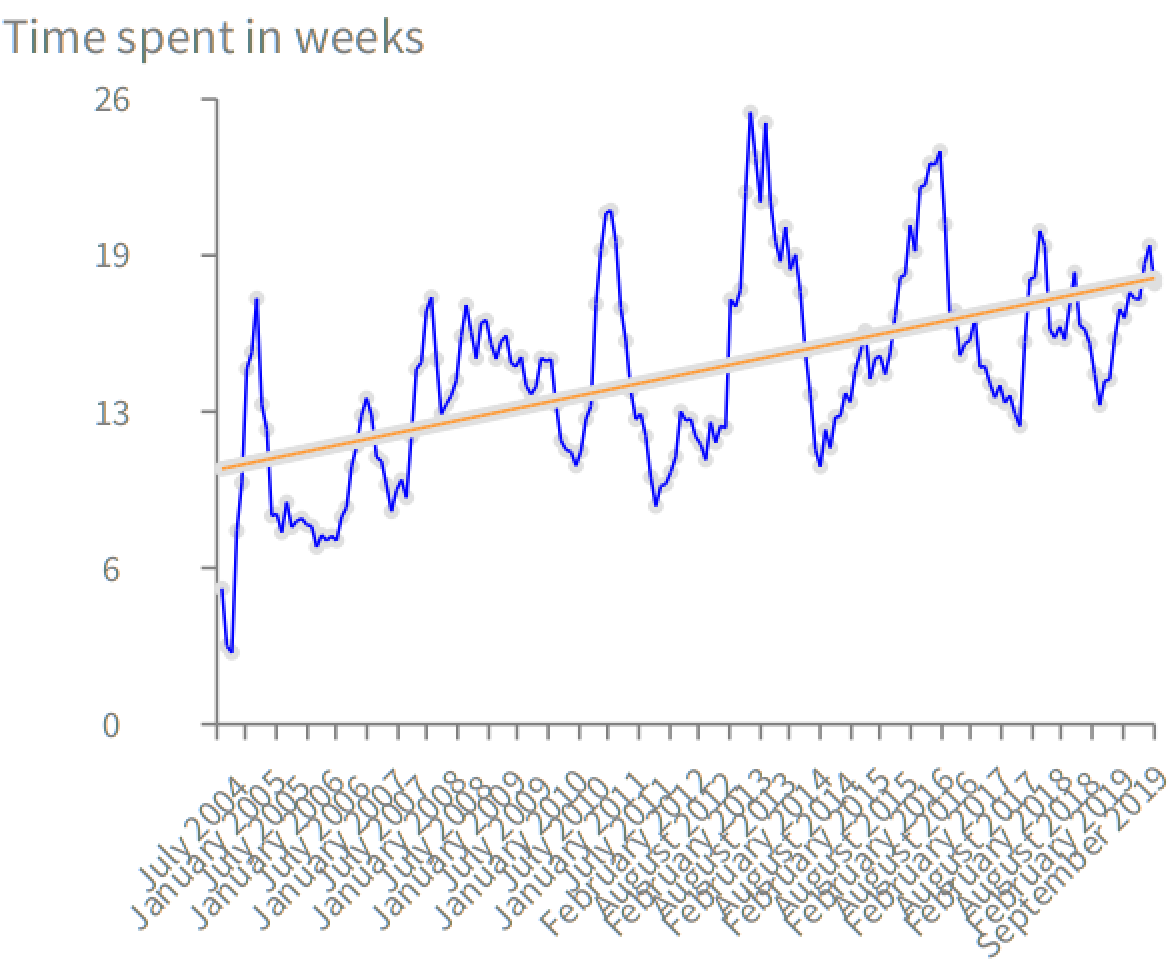
\includegraphics[width=70mm]{./images/openCloseEvol.png}
  \caption{Time to close evolution tickets}
  \label{fig:evol}
\end{figure}

\begin{figure}[H]
  \centering
  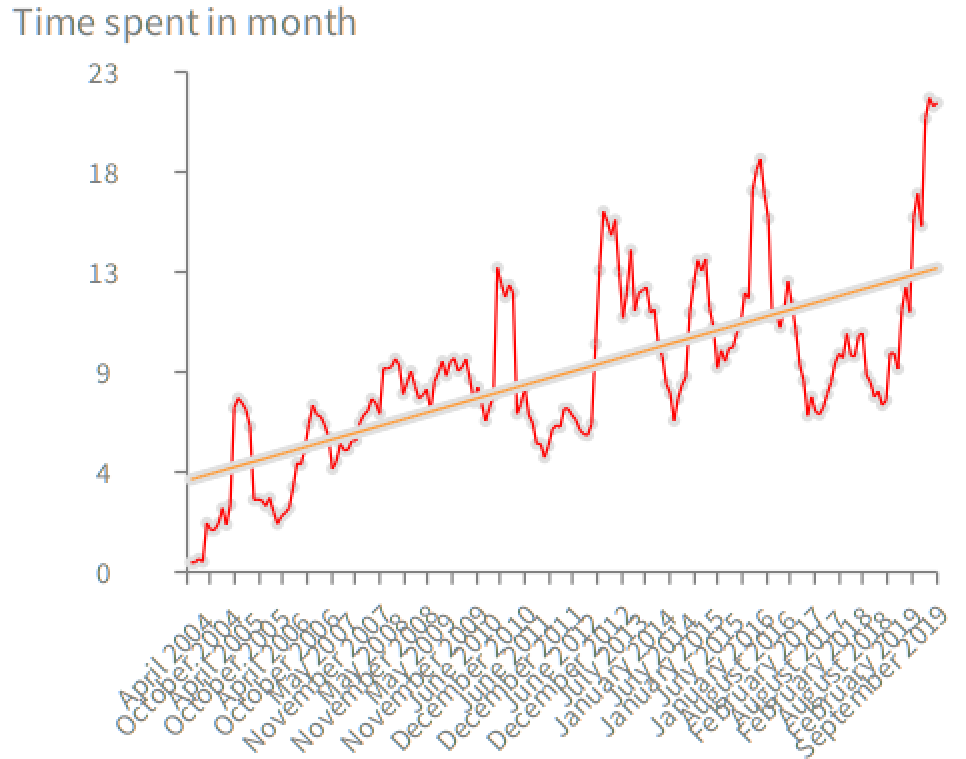
\includegraphics[width=70mm]{./images/openCloseBug.png}
  \caption{Time to close defects tickets}
  \label{fig:defect}
\end{figure}




\subsubsection{Time developer spend on a ticket }
%-------------------------------------------------------------------------------

When a developer work on the task assign to in a ticket, he spend time to analyse  the task. 
He then implement a solution and then test.
 The time spend analyzing and implementing the task assign in a ticket depend on the workload  of the ticket, the complexity of system, etc.  
We compute the average time spent by developers per month. 
The data also present rapid up-and-down variation, which we smooth with simple moving average of period 4. We use  linear regression to fit the data.   

\begin{figure}[H]
  \centering
  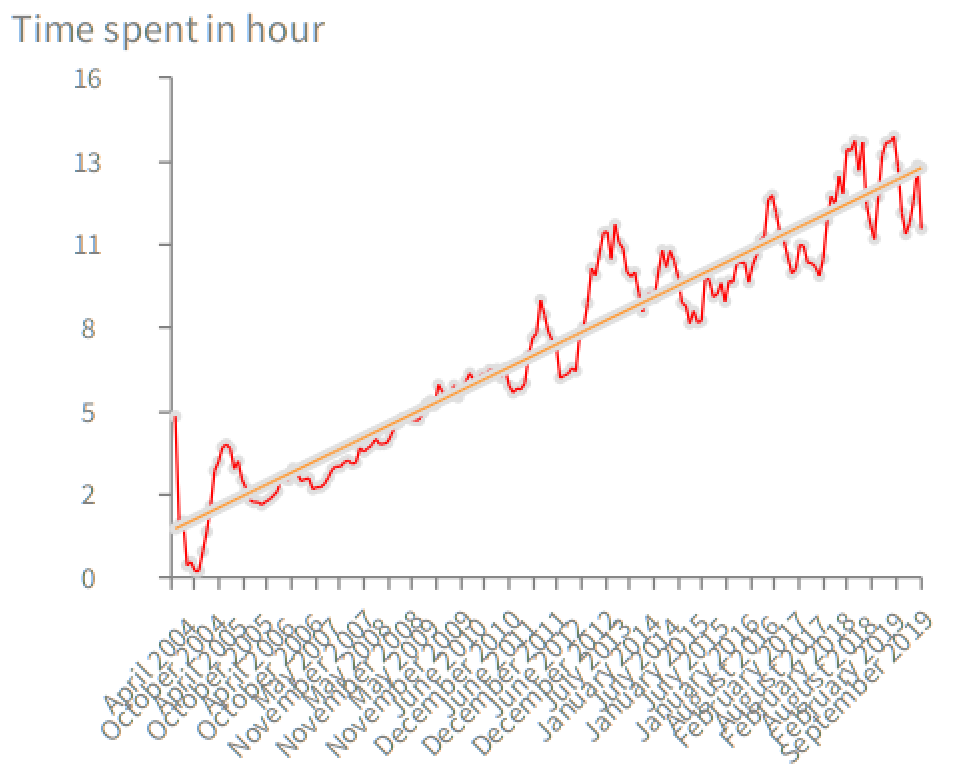
\includegraphics[width=70mm]{./images/devDefect.png}
  \caption{Time spent by a developer to implement solution for  defects tickets}
  \label{fig:devTimeDefect}
\end{figure}

\begin{figure}[H]
  \centering
  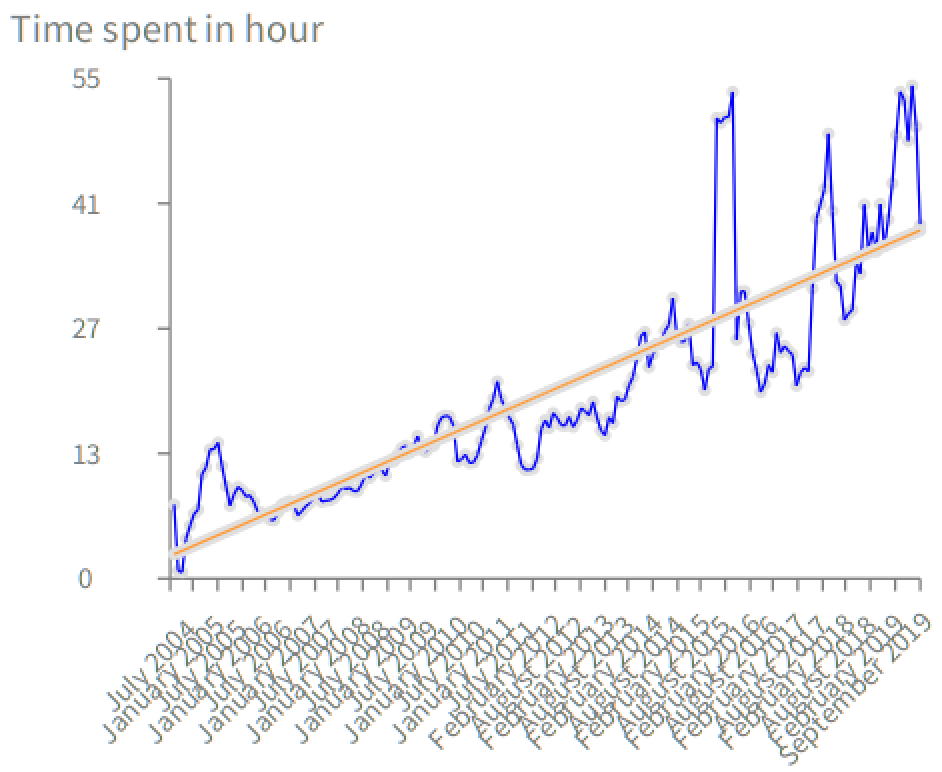
\includegraphics[width=70mm]{./images/devEvol.png}
  \caption{Time spent by a developer to implement solution for  evolution tickets}
  \label{fig:devTimeEvol}
\end{figure}

\subsubsection{Average time  to test a ticket after development}
%-------------------------------------------------------------------------------

Generally, when a developer finishes a development related to a ticket, he tests his solution.  
The testing time is recorded in the ticket database.
 We use this information to compute the average per month of testing time. 

 \begin{figure}[H]
  \centering
  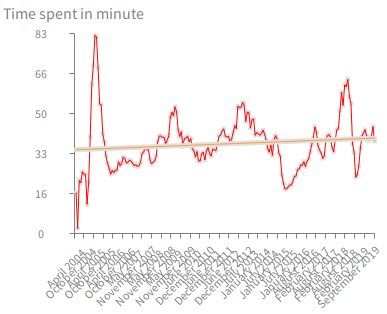
\includegraphics[width=70mm]{./images/timeDevTest.png}
  \caption{Time spent by a developer to test his solution for  defect tickets}
  \label{fig:devTimeTestBug}
\end{figure}

\begin{figure}[H]
  \centering
  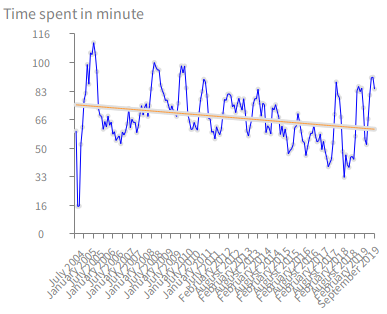
\includegraphics[width=70mm]{./images/evolutionTest.png}
  \caption{Time spent by a developer to test his solution for  evolution tickets}
  \label{fig:devTimeTestEvol}
\end{figure}

 \subsubsection{Team Manager time estimation}
 %-------------------------------------------------------------------------------

For a ticket, the team manager estimates the time needed to finish the task related to the ticket.
This estimation is based on the experience of the team manager.  
We compare the time spent by the developer with the estimation per month over the life cycle of the system.  
This is to assess if the developer has enough time to develop good quality source code.

\begin{figure}[H]
  \centering
  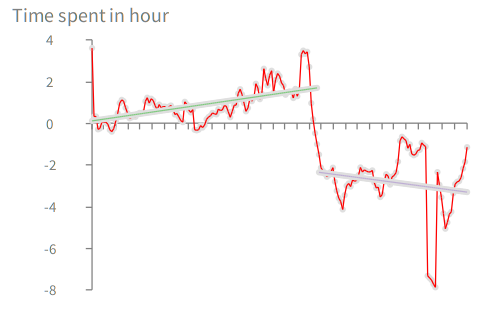
\includegraphics[width=70mm]{./images/estimateBug.png}
  \caption{Actual time spent by the developer minus time estimated by the manager for defect tickets.  The yAxis represent the value of the gap between the development time and the estimated time in hour. The xAxis represent months from 2004 to 2019}
  \label{fig:devEstDefect}
\end{figure}

\begin{figure}[H]
  \centering
  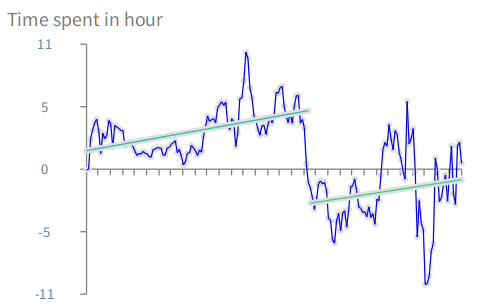
\includegraphics[width=70mm]{./images/estimateEvol.png}
  \caption{Actual time spent by the developer minus time estimated by the manager for evolution tickets. 
    The yAxis represent the value of the gap between the development time and the estimated time in hour. 
    The xAxis represent months from 2004 to 2019}
  \label{fig:devEstEvol}
\end{figure}

\section{Results and Discussion}
%-------------------------------------------------------------------------------
\label{sec:results-discussion}

\begin{itemize}
    \item Developers are now using subversion to integrate all their changes in the system. 
    \item From 2004 to 2019, as we can see in figure \ref{fig:evol} and figure \ref{fig:defect} ,  the time to close a ticket is 5 times the time at 2004 for defects and 1.5 times for evolution.
    \item Developers spend 4 times the time spent at 2004 for evolution tickets figure \ref{fig:devTimeEvol}, and  3 times for defects tickets figure \ref{fig:devTimeDefect}.
    \item  Figure \ref{fig:devTimeTestEvol} and \ref{fig:devTimeTestBug} show that the developer spend in average 45 minutes test  the feature implemented of the fixed defect.
    \item The time estimated by the developers team manager trend to be enough for the developer from 2013 for defects tickets and evolutions tickets.
\end{itemize}

\section{Summary and Conclusions}
%-------------------------------------------------------------------------------
\label{sec:conclusion}

In this paper we present our first step in  improving practices in a french company. We first introduce subversion, a version control system.
The developers team is now using it and the software studied source code is now versioned.
This open the door for further analysis of the code repository to understand the system evolution. 
Using the ticket database, the moving average and regression line, we build a defect model mainly assess the developer effort throughout the project life cycle. We will use this model to monitor our future actions which is: how to decompose the system big methods.
\bibliographystyle{plainnat}
%\bibliographystyle{alpha}
\bibliography{rmod,new}

\vspace{12pt}
\end{document}
